\subsection*{期末测试}
\setcounter{problemname}{0}

\begin{problem}
试写出进程映像包括哪些组成部分。
\end{problem}

\begin{solution}
进程控制块、进程程序块、进程数据块和进程核心栈。
\end{solution}


\begin{problem}
I/O软件的一般分为四层结构,请按照自顶向下的顺序写出四层结构的名称。
\end{problem}
    
\begin{solution}
    用户空间的I/O软件;独立于设备的I/O软件;设备驱动程序;中断处理程序。
\end{solution}


\begin{problem}
假设一个可移动磁头的磁盘具有200个磁道,编号为0$\sim$199,刚结束了175道的存取,正在处理143道的服务请求,假设系统当前I/O请求队列如下:85,145,90,180,92,150,102,176,132。试问:如果采用电梯调度算法完成上述请求,其存取臂移动的总量是多少?并写出磁头臂移动的序列。
\end{problem}

\begin{solution}
    磁头移动序列为132$\rightarrow$\,102$\rightarrow$\,92$\rightarrow$\,90$\rightarrow$\,85$\rightarrow$\,145$\rightarrow$\,150$\rightarrow$\,176$\rightarrow$\,180

    存取臂移动的总量为$(143-85)+(180-85)=153$
\end{solution}


\begin{problem}
请画出或描述出七状态进程模型(含两个挂起状态)及其状态转换图。
\end{problem}

\begin{solution}
    \begin{figure}[H]
        \vspace{-0.5em}
        \centering
        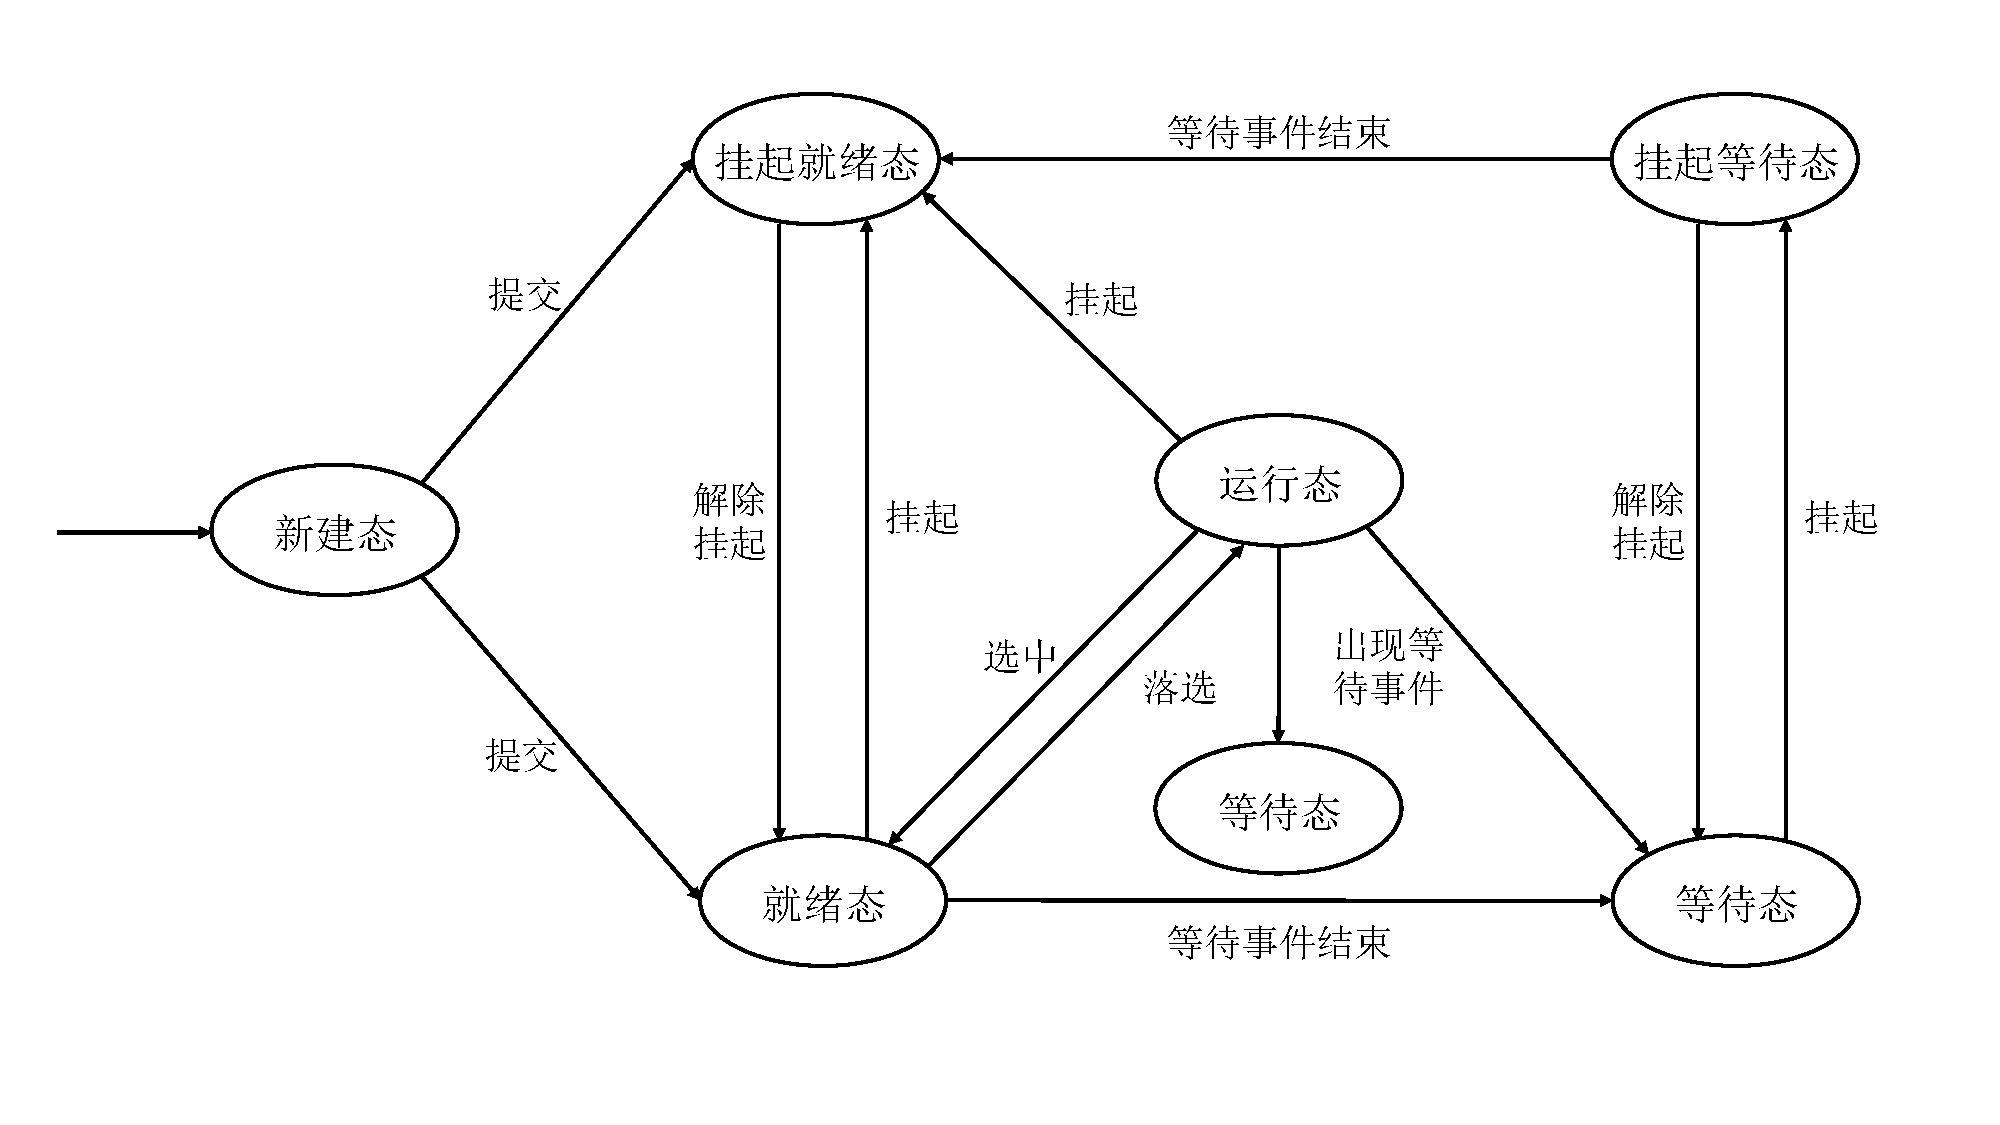
\includegraphics[width=0.7\linewidth]{七状态进程模型.pdf}
        \vspace{-1em}
    \end{figure}
\end{solution}



\begin{problem}
一台机器有48位虚地址和32位物理地址,若页长为4KB,问如果采用正向页表,一个进程的页表最多有多少个页表项? 如果设计一个反置页表,则有多少个页表项?
\end{problem}

\begin{solution}
    由于页长为4KB($2^{12}$B),所以页内偏移量为12位,所以页表项共有$2^{48-12}=2^{36}$个,反置页表项共有$2^{32-12}=2^{20}$个。
\end{solution}


\begin{problem}
 在UNIX系统中,每个$i$节点中分别含有12个直接地址的索引和一、二、三级间接索引。假设每个盘块有1024Byte,若每个盘块放256个盘块地址,50MB的文件和100MB的文件分别占用多少直接、一、二、三级间接盘块?
\end{problem}

\begin{solution}
直接盘块容量:$1024\mathrm{B}\times 12=12\mathrm{KB}$

一级间接盘块容量:$256 \times 1024\mathrm{B}=256\mathrm{KB}$

二级间接盘块容量:$256 \times 256\mathrm{KB}=65536\mathrm{KB}=64\mathrm{MB}$

三级间接盘块容量:$64\mathrm{MB} \times 256=16384\mathrm{MB}$

50MB的文件占用12个直接盘块和256个一级间接盘块,二级间接盘块占用数量为$(50\mathrm{MB}-12\mathrm{KB}-256\mathrm{KB})\div 1024\mathrm{B}=50932$个

100MB的文件占用12个直接盘块、256个一级间接盘块和$256\times 256=65536$个二级间接盘块,三级间接盘块的占用数量为$(100\mathrm{MB}-12\mathrm{KB}-256\mathrm{KB}-64\mathrm{MB})\div 1024\mathrm{B}=36596$个

\end{solution}


\begin{problem}
考虑下面的进程集合:
\begin{table}[H]
    \vspace{-0.5em}
    \centering
    \begin{tabular}{|c|c|c|}
    \hline
    进程& 到达时间& 处理时间\\ \hline
    A & 0   & 2   \\ \hline
    B & 1   & 8   \\ \hline
    C & 2   & 2   \\ \hline
    D & 3   & 8   \\ \hline
    \end{tabular}
    \vspace{-1.5em}
\end{table}
如果使用先来先服务FCFS调度算法,得到的每个单位时间内的进程执行序列表示为:
\begin{table}[H]
    \vspace{-0.5em}
    \centering
    \resizebox{\linewidth}{!}{
    \begin{tabular}{|c|c|c|c|c|c|c|c|c|c|c|c|c|c|c|c|c|c|c|c|c|}
    \hline
    算法  & 1   & 2   & 3   & 4   & 5   & 6   & 7   & 8   & 9   & 10  & 11  & 12  & 13  & 14  & 15  & 16  & 17  & 18  & 19  & 20  \\ \hline
    FCFS & A & A & B & B & B & B & B & B & B & B & C & C & D & D & D & D & D & D & D & D \\ \hline
    \end{tabular}
    }
    \vspace{-1.5em}
\end{table}
参照该FCFS调度算法给出的执行序列的写法,写出如果采用时间片轮转RR(时间片单位$q=1, q=4$)、多级反馈队列Feedback(反馈Fback,$q=1$;Fback,$q=2^i$)等4个调度算法,得到进程执行序列。注:在时间片轮转或者多级反馈队列调度时,如果就绪队列都为空,正在运行的进程不被抢占,继续使用下一段时间片。

\end{problem}

\begin{solution}
    \begin{table}[H]
        \vspace{-0.5em}
        \centering
        \resizebox{\linewidth}{!}{
        \begin{tabular}{|c|c|c|c|c|c|c|c|c|c|c|c|c|c|c|c|c|c|c|c|c|}
        \hline
        算法          & 1    & 2    & 3    & 4    & 5    & 6    & 7    & 8    & 9    & 10   & 11   & 12   & 13   & 14   & 15   & 16   & 17   & 18   & 19   & 20   \\ \hline
        RR,$q=1$     &  A  & B  &  A &  C &  B &  D &  C &  B &  D & B  &  D &  B &  D &  B &  D &  B & D  &  B &  D &  D \\ \hline
        RR,$q=4$     & A  & A  &  B &  B &  B &  B &  C &  C &  D &  D &  D &  D &  B & B  &  B &  B &  D &  D &  D &  D \\ \hline
        Fback,$q=1$  &  A &  B &  C &  D &  A &  B &  C & D  & B  &  D &  B &  D &  B &  D &  B &  D &  B &  D &  B & D  \\ \hline
        Fback,$q=2^i$ & A  &  B &  C &  D & A  &  B &  B &  C &  D &  D &  B &  B &  B &  B &  D &  D &  D &  D &  B & D    \\ \hline
        \end{tabular}
        }
        \vspace{-1.5em}
        \end{table}
\end{solution}



\begin{problem}
假设一个进程在磁盘上包含6个虚拟页(0号$\sim$5号),在主存中固定分配给3个页框,发生如下顺序的页访问:4, 3, 2, 1, 4, 3, 5, 4, 3, 2, 1, 5   
\begin{enumerate}[label=(\arabic*)]
    \item 如果使用LRU策略,给出相继驻留在这3个帧上的页。计算主存的缺页次数。
    \item 如果使用Clock策略,给出相继驻留在这3个帧上的页。计算主存的缺页次数。
\end{enumerate}

\end{problem}

\begin{solution}
    LRU算法:缺页次数为10次。
    \begin{table}[H]
        \centering
        \vspace{-0.5em}
        \begin{tabular}{rcccccccccccc}
        \multicolumn{1}{c}{}     & 4                      & 3                      & 2                      & 1                      & 4                      & 3                      & 5                      & 4                      & 3                      & 2                      & 1                      & 5                      \\ \cline{2-13} 
        \multicolumn{1}{r|}{页框0} & \multicolumn{1}{c|}{4} & \multicolumn{1}{c|}{4} & \multicolumn{1}{c|}{4} & \multicolumn{1}{c|}{1} & \multicolumn{1}{c|}{1} & \multicolumn{1}{c|}{1} & \multicolumn{1}{c|}{5} & \multicolumn{1}{c|}{5} & \multicolumn{1}{c|}{5} & \multicolumn{1}{c|}{2} & \multicolumn{1}{c|}{2} & \multicolumn{1}{c|}{2} \\ \cline{2-13} 
        \multicolumn{1}{r|}{页框1} & \multicolumn{1}{c|}{}  & \multicolumn{1}{c|}{3} & \multicolumn{1}{c|}{3} & \multicolumn{1}{c|}{3} & \multicolumn{1}{c|}{4} & \multicolumn{1}{c|}{4} & \multicolumn{1}{c|}{4} & \multicolumn{1}{c|}{4} & \multicolumn{1}{c|}{4} & \multicolumn{1}{c|}{4} & \multicolumn{1}{c|}{1} & \multicolumn{1}{c|}{1} \\ \cline{2-13} 
        \multicolumn{1}{r|}{页框2} & \multicolumn{1}{c|}{}  & \multicolumn{1}{c|}{}  & \multicolumn{1}{c|}{2} & \multicolumn{1}{c|}{2} & \multicolumn{1}{c|}{2} & \multicolumn{1}{c|}{3} & \multicolumn{1}{c|}{3} & \multicolumn{1}{c|}{3} & \multicolumn{1}{c|}{3} & \multicolumn{1}{c|}{3} & \multicolumn{1}{c|}{3} & \multicolumn{1}{c|}{5} \\ \cline{2-13} 
        缺页标记                     & F                      & F                      & F                      & F                      & F                      & F                      & F                      &                        &                        & F                      & F                      & F                     
        \end{tabular}
        \vspace{-1.5em}
        \end{table}
    Clock算法:缺页次数为9次。
    \begin{table}[H]
        \centering
        \vspace{-0.5em}
        \begin{tabular}{rcccccccccccc}
        \multicolumn{1}{c}{}     & 4                                  & 3                                  & 2                                    & 1                                   & 4                                   & 3                                    & 5                                   & 4                                    & 3                                    & 2                                   & 1                                   & 5                                    \\ \cline{2-13} 
        \multicolumn{1}{r|}{页框0} & \multicolumn{1}{c|}{4*}            & \multicolumn{1}{c|}{4*}            & \multicolumn{1}{c|}{$\rightarrow$\,4*} & \multicolumn{1}{c|}{1*}             & \multicolumn{1}{c|}{1*}             & \multicolumn{1}{c|}{$\rightarrow$\,1*} & \multicolumn{1}{c|}{5*}             & \multicolumn{1}{c|}{5*}              & \multicolumn{1}{c|}{5*}              & \multicolumn{1}{c|}{5}              & \multicolumn{1}{c|}{$\rightarrow$\,5} & \multicolumn{1}{c|}{$\rightarrow$\,5*} \\ \cline{2-13} 
        \multicolumn{1}{r|}{页框1} & \multicolumn{1}{c|}{$\rightarrow$\,} & \multicolumn{1}{c|}{3*}            & \multicolumn{1}{c|}{3*}              & \multicolumn{1}{c|}{$\rightarrow$\,3} & \multicolumn{1}{c|}{4*}             & \multicolumn{1}{c|}{4*}              & \multicolumn{1}{c|}{$\rightarrow$\,4} & \multicolumn{1}{c|}{$\rightarrow$\,4*} & \multicolumn{1}{c|}{$\rightarrow$\,4*} & \multicolumn{1}{c|}{2*}             & \multicolumn{1}{c|}{2*}             & \multicolumn{1}{c|}{2*}              \\ \cline{2-13} 
        \multicolumn{1}{r|}{页框2} & \multicolumn{1}{c|}{}              & \multicolumn{1}{c|}{$\rightarrow$\,} & \multicolumn{1}{c|}{2*}              & \multicolumn{1}{c|}{2}              & \multicolumn{1}{c|}{$\rightarrow$\,2} & \multicolumn{1}{c|}{3*}              & \multicolumn{1}{c|}{3}              & \multicolumn{1}{c|}{3}               & \multicolumn{1}{c|}{3*}              & \multicolumn{1}{c|}{$\rightarrow$\,3} & \multicolumn{1}{c|}{1*}             & \multicolumn{1}{c|}{1*}              \\ \cline{2-13} 
        缺页标记                     & F                                  & F                                  & F                                    & F                                   & F                                   & F                                    & F                                   &                                      &                                      & F                                   & F                                   &                                     
        \end{tabular}
        \vspace{-1.5em}
    \end{table}
\end{solution}


\begin{problem}
    设系统中有3种类型的资源(A、B、C)和5个进程(P1、P2、P3、P4、P5),A资源的总量为17,B资源的总量为5,C资源的总量为20。在$T_0$时刻系统状态如下表所示,系统采用银行家算法实施死锁避免策略。  
    \begin{figure}[H]
        \vspace{-0.5em}
        \centering
        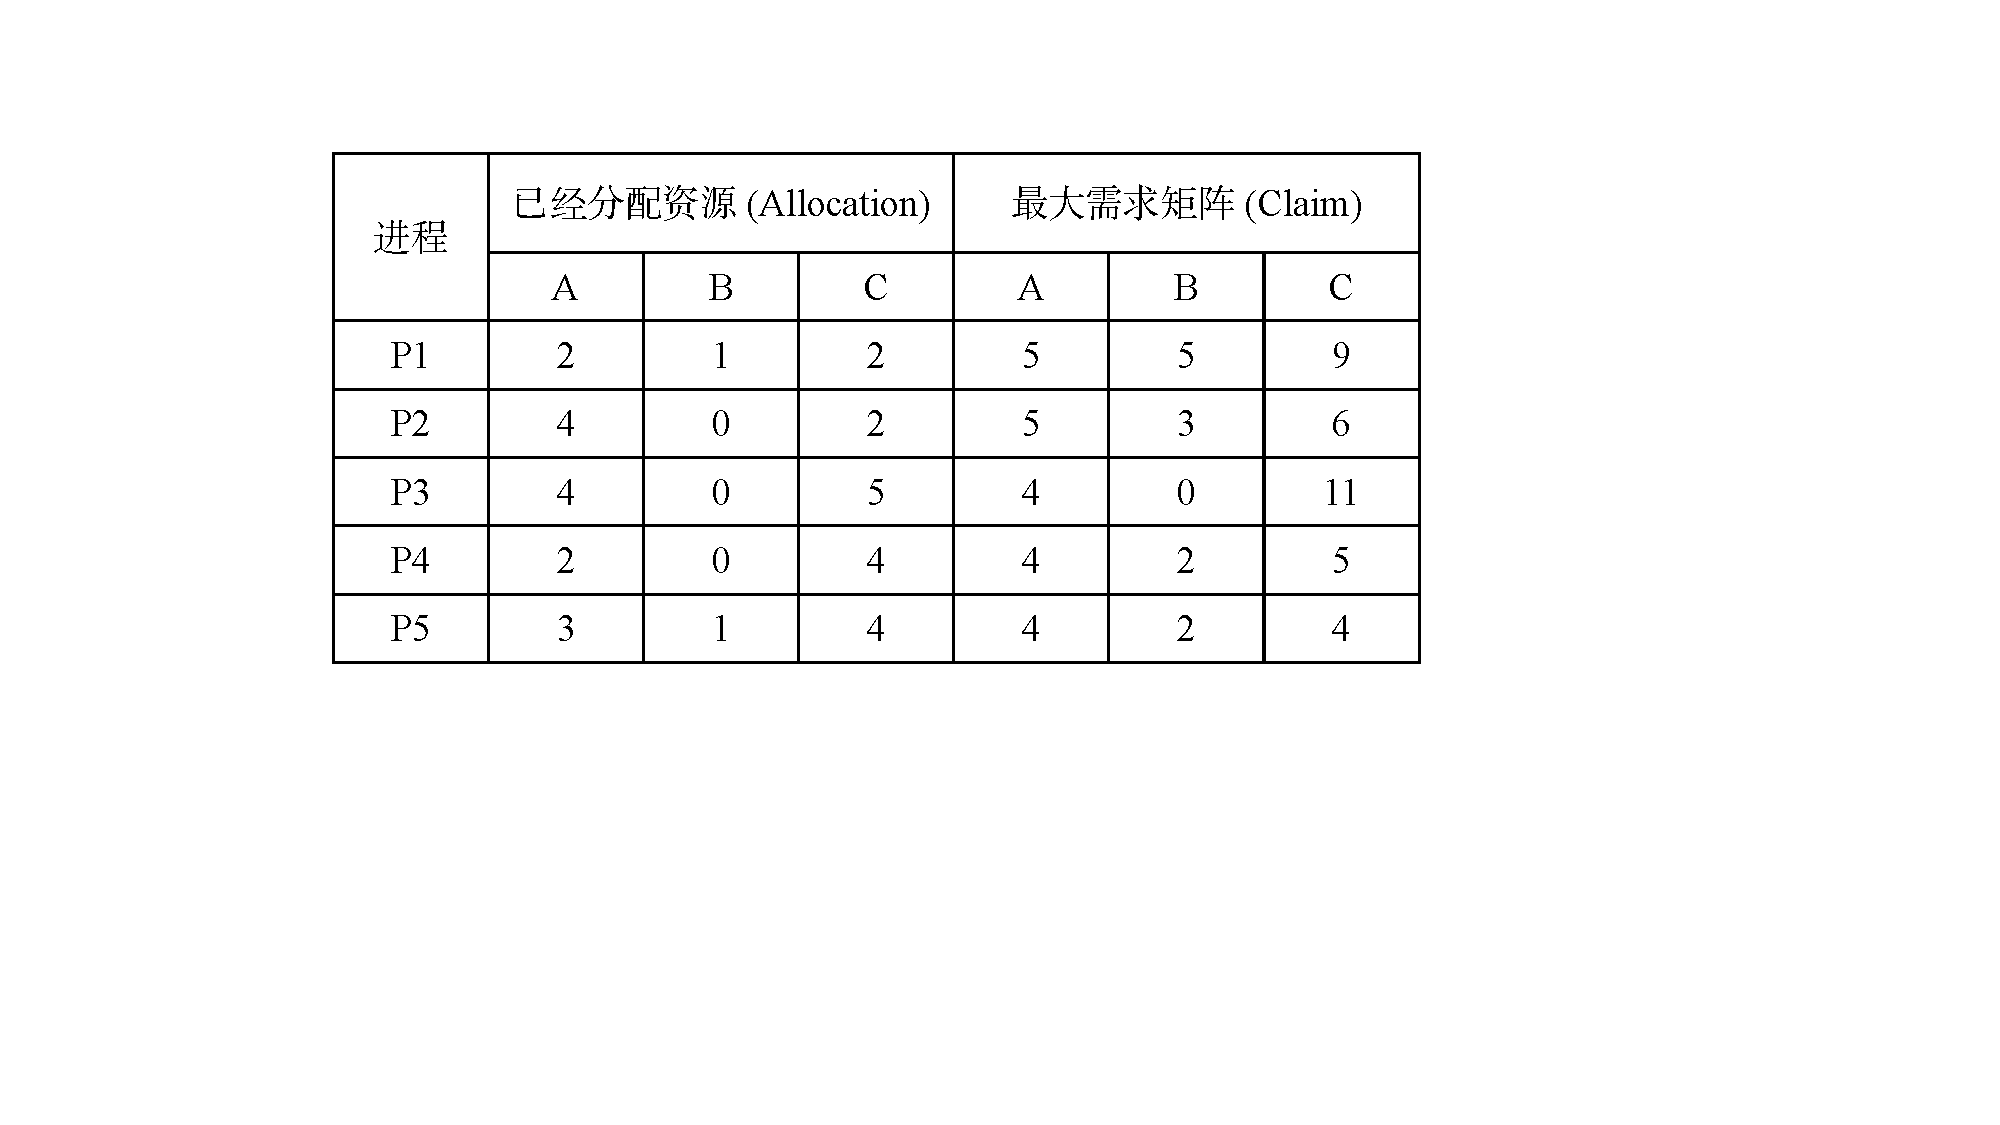
\includegraphics[width=0.5\linewidth]{期末考试第9题图.pdf}
        \vspace{-1em}
    \end{figure}
    \begin{enumerate}[label=(\arabic*)]
        \item $T_0$时刻的各资源剩余数量为多少?$T_0$时刻的是否为安全状态? 若是,请给出其中可能的一种安全序列,并依照该序列,写出各资源的回收步骤。
        \item 在$T_0$时刻,如果进程P1继续对A、B、C三类资源提出请求$Request(2, 2, 2)$后,系统能否将资源分配给P1进程?给出理由。
    \end{enumerate}

    
\end{problem}
    
\begin{solution}
    $T_0$时刻A资源的剩余量为$17-2-4-4-2-3=2$,B资源的剩余量为$5-1-1=3$,C资源的剩余量为$20-2-2-5-4-4=3$。

    $T_0$时刻为安全状态,其中的可能安全序列为P4$\rightarrow$P2$\rightarrow$P3$\rightarrow$P5$\rightarrow$P1

    \begin{figure}[H]
        \vspace{-0.5em}
        \centering
        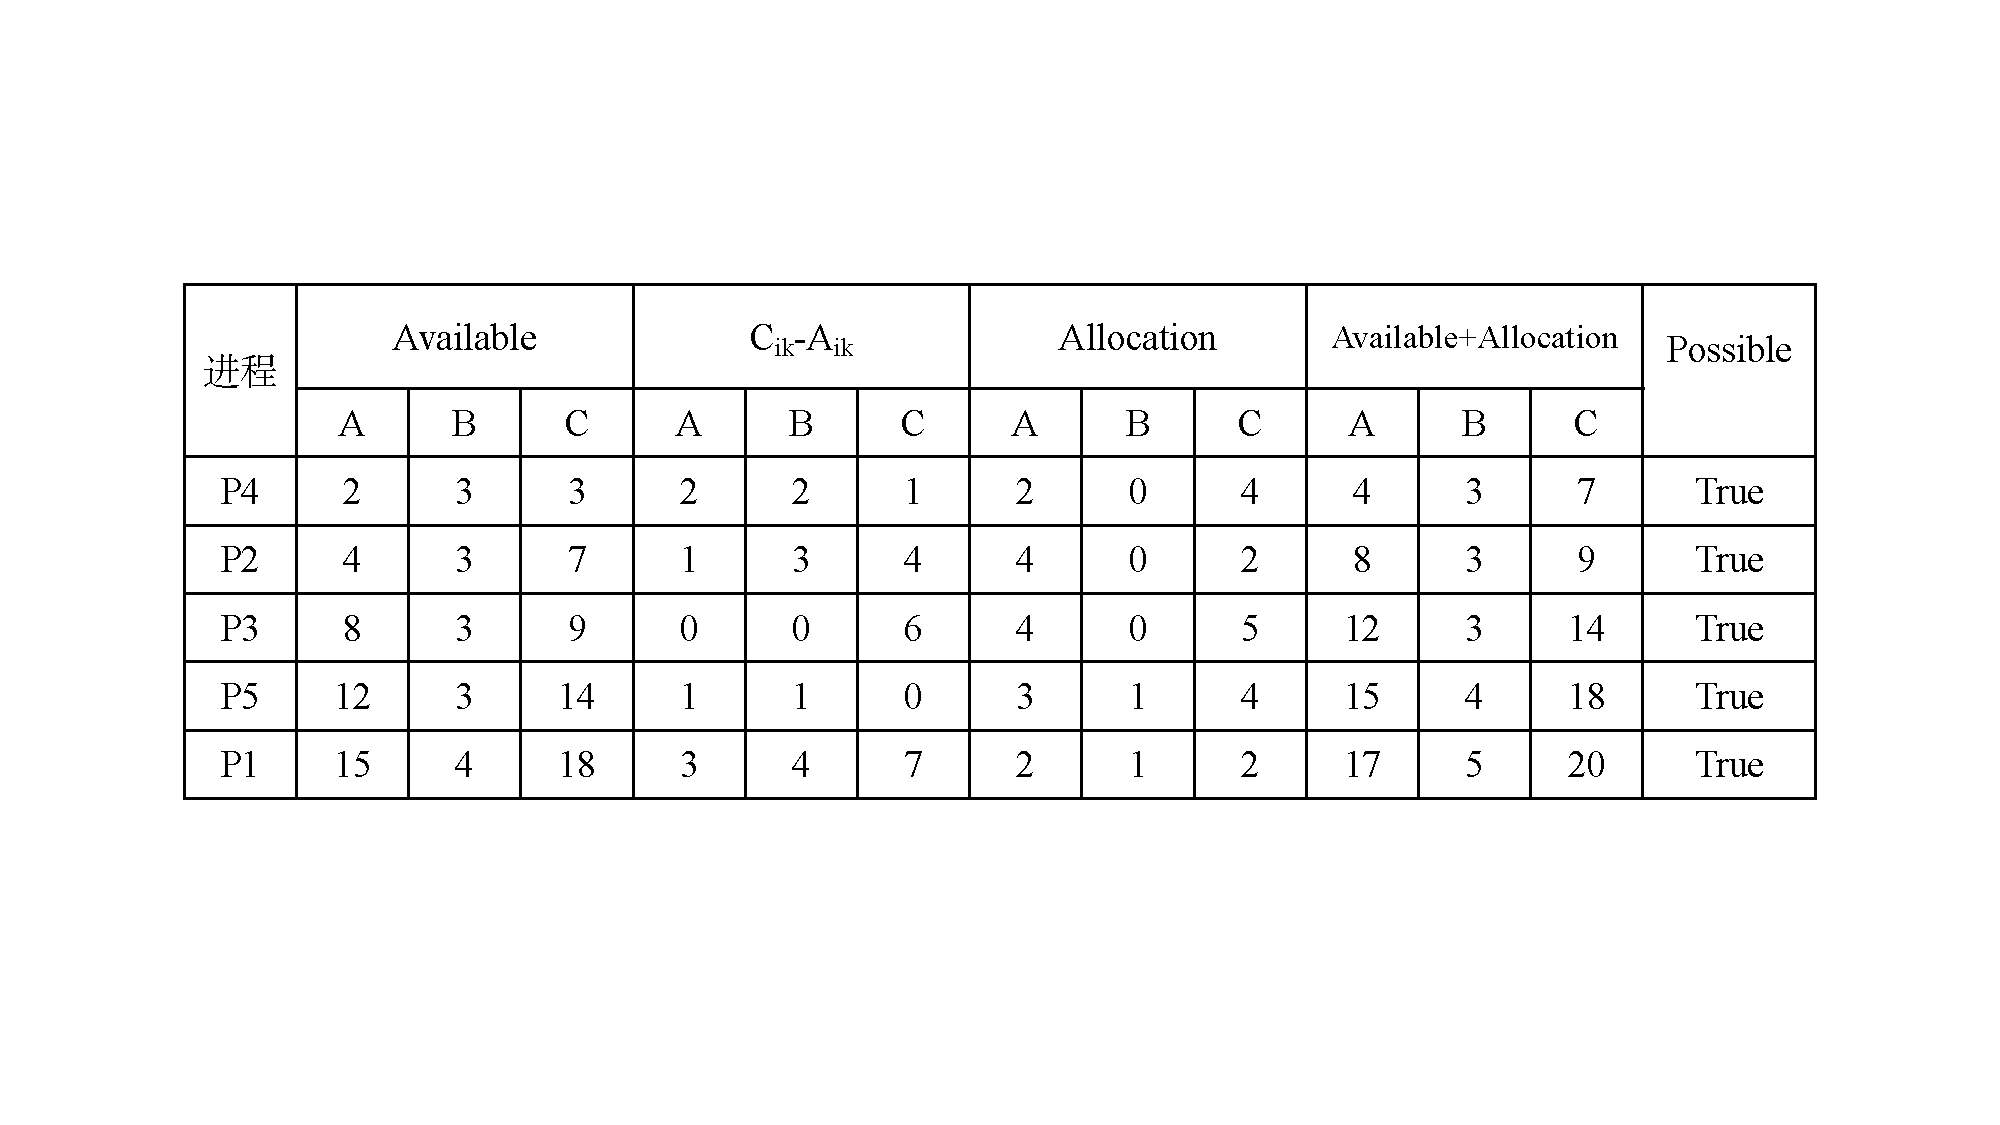
\includegraphics[width=0.8\linewidth]{期末考试第9题答案图.pdf}
        \vspace{-1em}
    \end{figure}

    在$T_0$时刻,假设满足P1的分配需求,此时$Available=(0,1,1)$,不能满足任何一个进程,系统处于不安全状态,因此不能分配。
\end{solution}

